\documentclass{standalone}

\usepackage{amsmath}
\usepackage{unicode-math}
\usepackage{tikz}
\usepackage{circuitikz}

\usetikzlibrary{
  patterns, patterns.meta,
  arrows, arrows.meta,
  bending,
  positioning,
  decorations.markings, decorations.pathreplacing,
  shapes.misc, shapes.geometric
}
\tikzset{
  dot/.style = {circle, fill=red!80!gray, minimum
      size=#1, draw=black,
      inner sep=0pt, outer sep=0pt},
  dot/.default = 5pt, % size of the circle diameter
  gdot/.style = {dot=#1, fill=white},
  bdot/.style = {dot=#1, fill=black},
  gdot/.default = 5pt, % size of the circle diameter
  bdot/.default = 5pt, % size of the circle diameter
  extended line/.style={shorten >=-#1,shorten <=-#1},
  extended line/.default=3mm,
  rod/.style={double distance=#1, line cap=round, very thick,
      double=gray!20},
  rod/.default=4mm,
  var/.style={rectangle, fill=white},
  guide/.style={gray, line width=.6pt},
  dim/.style={latex-latex, teal, thick},
  edge/.style={
      postaction=decorate, decoration={
	  markings,
	  mark=at position #1 with {\arrow{Latex[round, length=3mm, bend]}}
	}
    },
  edge/.default=.55,
  generator/.style={midway, gdot=#1, fill opacity=0},
  generator/.default=10mm,
}

\begin{document}
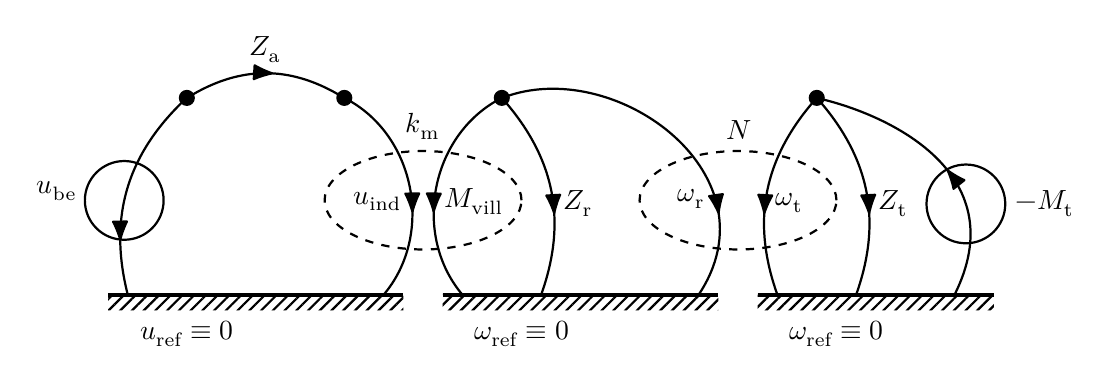
\begin{tikzpicture}[thick, scale=1]
  \node[bdot] (ug) at (0,2.5) {};
  \node[bdot] (ube) at (2,2.5) {};
  \node[bdot] (wki) at (4,2.5) {};
  \node[bdot] (wbe) at (8,2.5) {};

  \draw[ultra thick]
  (-1, 0) -- (2.75, 0)
  (3.25, 0) -- (6.75, 0)
  (7.25, 0) -- (10.25,0)
  ;
  \fill[pattern = {Lines[angle=45,distance={3pt}]}]
  (-1, 0) rectangle (2.75, -.20)
  (3.25, 0) rectangle (6.75, -.20)
  (7.25, 0) rectangle (10.25,-.20)
  ;

  \draw[edge=.74] (ug) to[bend right] node[generator, pos=.55] {} node[left=5mm] {$u_\text{be}$} (-.75,0);
  \draw[edge=.55] (ug) to[bend left] node [midway, above] {$Z_\text{a}$} (ube);
  \draw[edge=.60] (ube) to[bend left=50] node[left, pos=.55] {$u_\text{ind}$} (2.5,0);

  \draw[edge=.60] (wki) to[bend right=50] node[right, pos=.55] {$M_\text{vill}$} (3.5,0);
  \draw[edge=.60] (wki) to[bend left] node[right, pos=.55] {$Z_\text{r}$} (4.5,0);
  \draw[edge=.76] (wki) .. controls (5.5,3) and (7.5,1.5) .. node[left, pos=.72] {$\omega_\text{r}$} (6.5,0);

  \draw[edge=.60] (wbe) to[bend right] node[right, pos=.55] {$\omega_\text{t}$} (7.5,0);
  \draw[edge=.60] (wbe) to[bend left] node[right, pos=.55] {$Z_\text{t}$} (8.5,0);
  \draw[edge=.48] (9.75,0) .. controls (10.5,1.5) and (9,2.25) ..
  node[generator, pos=.3] {} node [right=5mm, pos=.30] {$-M_\text{t}$} (wbe);

  \node[ellipse, draw=black, minimum width = 2.5cm, minimum height=1.25cm, dashed] (ell1) at (3,1.2) {};
  \node[ellipse, draw=black, minimum width = 2.5cm, minimum height=1.25cm, dashed] (ell2) at (7,1.2) {};
  \node[above] at (ell1.north) {$k_\text{m}$};
  \node[above] at (ell2.north) {$N$};

  \node at (0,-.5) {$u_\text{ref} \equiv 0$};
  \node at (4.25,-.5) {$\omega_\text{ref} \equiv 0$};
  \node at (8.25,-.5) {$\omega_\text{ref} \equiv 0$};
\end{tikzpicture}
\end{document}
